\chapter{TRIỂN KHAI VÀ VẬN HÀNH}

Chương 4. TRIỂN KHAI VÀ VẬN HÀNH

\section{Môi trường triển khai}

Dịch vụ N2 được triển khai trên một máy chủ ảo (VPS) với cấu hình như sau:

Bảng 4.1 Cấu hình VPS triển khai

Thành phần Thông số Hệ điều hành Windows Server 2022 CPU 4 vCPU Intel Xeon RAM 8 GB Ổ cứng 100 GB SSD Băng thông 100 Mbps Địa chỉ IP 163.223.210.87

\paragraph{Hệ thống sử dụng Docker để đóng gói và vận hành các service trong môi trường}

container hóa, đảm bảo tính nhất quán giữa môi trường phát triển và môi trường production.

\paragraph{Mỗi service được đóng gói trong một Docker image riêng và chạy trong container độc lập,}

\paragraph{kết nối với nhau qua Docker network nội bộ.}

\section{Docker hóa dịch vụ}

\subsection{Dockerfile}

\paragraph{Backend N2 được đóng gói bằng Docker image dựa trên ASP.NET Core runtime image}

\paragraph{chính thức của Microsoft. Dockerfile sử dụng kỹ thuật multi-stage build để tối ưu kích}

thước image: stage đầu tiên sử dụng SDK image để biên dịch mã nguồn, stage thứ hai chỉ chứa runtime và các file đã build, giúp giảm kích thước image cuối cùng xuống dưới 200 MB.

FROM mcr.microsoft.com/dotnet/aspnet:8.0 AS base WORKDIR /app EXPOSE 80

FROM mcr.microsoft.com/dotnet/sdk:8.0 AS build

WORKDIR /src COPY ["N2.Circulation.Api.csproj", "./"] RUN dotnet restore COPY . . RUN dotnet build ‐c Release ‐o /app/build

FROM build AS publish RUN dotnet publish ‐c Release ‐o /app/publish

FROM base AS final WORKDIR /app COPY ‐‐from=publish /app/publish . ENTRYPOINT ["dotnet", "N2.Circulation.Api.dll"]

\subsection{Docker Compose}

\paragraph{Toàn bộ hệ thống ba service cùng API Gateway được điều phối qua Docker Compose, cho}

phép khởi động toàn bộ hệ thống chỉ với một lệnh duy nhất. File cấu hình Compose định nghĩa network nội bộ, volume cho dữ liệu và các biến môi trường cần thiết.

services: n2‐circulation: image: n2‐circulation:latest container\_name: library\_circulation\_service ports: ‐ "5082:80" environment: ‐ ASPNETCORE\_HTTP\_PORTS=80 ‐ Jwt\_\_Key=<shared‐secret‐key> ‐ CatalogService\_\_BaseUrl=http://n1‐catalog ‐ IdentityService\_\_BaseUrl=http://n3‐identity networks: ‐ library‐network restart: unless‐stopped

\begin{itemize}
  \item Tạo Git checkpoint: Commit thay đổi lên một branch riêng, push lên GitHub và
tạo tag để có thể rollback nhanh nếu cần.

\end{itemize}

\begin{itemize}
  \item Deploy lên VPS: Copy các file build output hoặc pull Docker image mới lên VPS.
Đối với static UI, xóa thư mục UI cũ hoàn toàn trước khi copy bản mới — tuyệt đối không ghi đè chồng lấp.

\end{itemize}

\begin{itemize}
  \item Kiểm tra sau deploy: Xác nhận giao diện và API hoạt động bình thường trên VPS
thông qua trình duyệt và các lệnh curl.

\end{itemize}

\begin{itemize}
  \item Duy trì khả năng rollback: Luôn giữ lại tag hoặc commit hash của phiên bản trước
đó để có thể khôi phục nhanh trong trường hợp phiên bản mới gặp sự cố.

\end{itemize}

\section{Giám sát và health check}

Trong quá trình vận hành, nhóm sử dụng một số cơ chế giám sát cơ bản: Health check endpoint: Mỗi service cung cấp endpoint /ping trả về trạng thái hoạt động. Đây là endpoint đơn giản nhất để kiểm tra service còn sống hay không mà không cần xác thực.

\paragraph{Logging tập trung: Backend N2 ghi log tất cả các request đến (method, path,}

host) ra console thông qua middleware được cấu hình trong Program.cs. Trong môi trường

\paragraph{Docker, các log này được thu thập qua Docker logging driver và có thể truy xuất bằng lệnh}

docker logs. Kiểm tra định kỳ: Nhóm thực hiện kiểm tra thủ công định kỳ các service trên VPS, đặc biệt sau các đợt bảo trì hoặc cập nhật từ nhóm khác, để đảm bảo toàn bộ hệ thống vẫn hoạt động ổn định. Hướng phát triển: Trong tương lai, hệ thống có thể được bổ sung Prometheus + Grafana để giám sát chuyên sâu hơn (CPU, memory, request rate, error rate) và ELK Stack (Elasticsearch, Logstash, Kibana) để phân tích log tập trung.

\clearpage
\section*{H?nh ?nh v? s? ?? minh h?a}
\addcontentsline{toc}{section}{H?nh ?nh v? s? ?? minh h?a}
\begin{figure}[H]
\centering
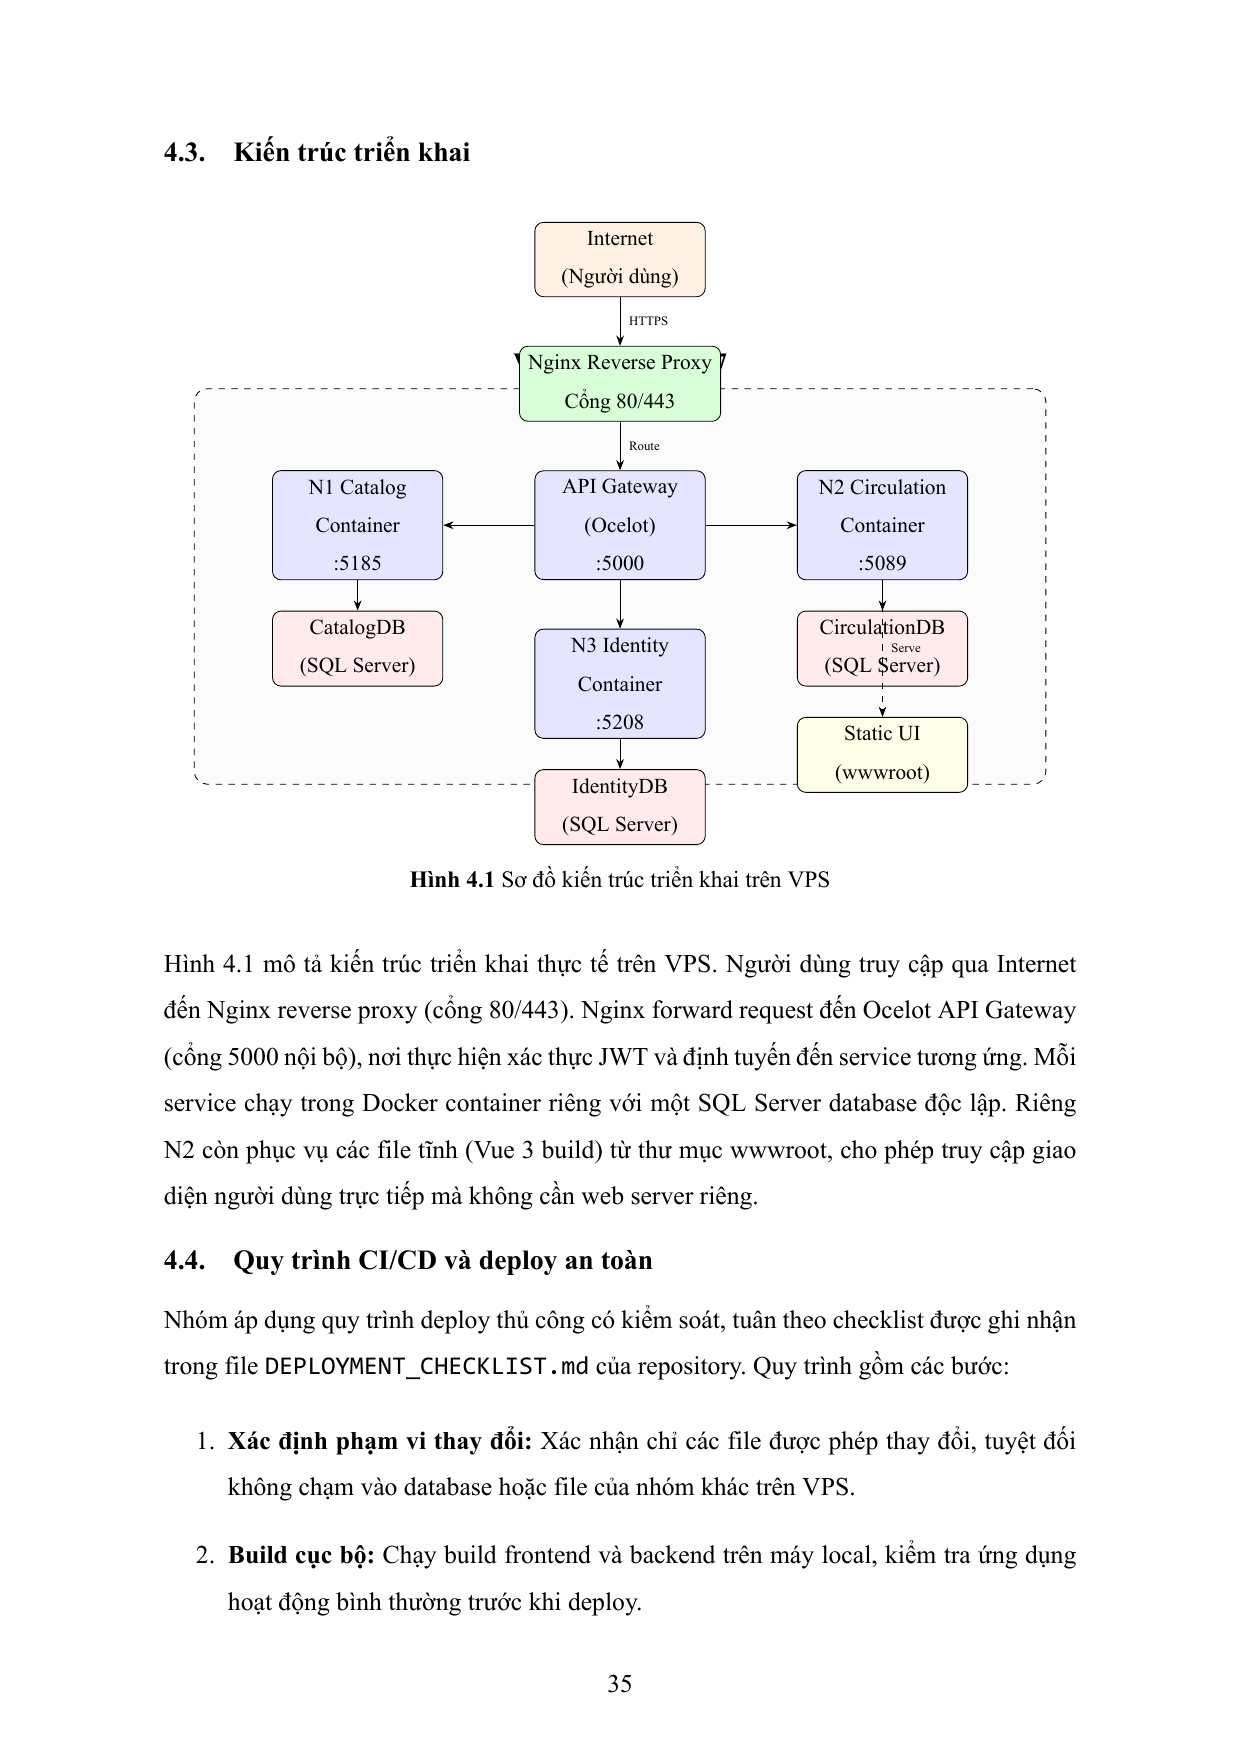
\includegraphics[width=0.98\textwidth]{figures/fig-48-48.png}
\caption{H?nh ?nh/s? ?? tr?ch t? b?o c?o g?c, trang 48}
\end{figure}
\clearpage
